\chapter{Технологическая часть}

\section{Средства реализации}

Для программной реализации шифровальной машины был выбран язык Rust. В данном языке есть все требующиеся инструменты для данной лабораторной работы.

\section{Реализация алгоритма}

В листингах~\ref{lst:reflector}~---~\ref{lst:enigma} представлена реализация шифровальной машины Энигма.

\begin{center}
\captionsetup{justification=raggedright,singlelinecheck=off}
\begin{lstlisting}[label=lst:reflector,caption=реализация рефлектора]
pub struct Reflector<T> {
    alphabet: Vec<T>,
}

impl<T: Clone + Eq> Reflector<T> {
    pub fn from_alphabet(alphabet: &[T]) -> Result<Self, &str> {
        if alphabet.len() % 2 != 0 {
            return Err("Error: Can't be odd alphabet");
        }
        let mut rng = rng();
        let mut cipher = alphabet.to_vec();
        cipher.shuffle(&mut rng);

        Ok(Reflector { alphabet: cipher })
    }

    pub fn from_config(config: &[T]) -> Result<Self, &str> {
        if config.len() % 2 != 0 {
            return Err("Error: Can't be odd alphabet");
        }

        Ok(Reflector {
            alphabet: config.to_vec(),
        })
    }

    pub fn get_config(&self) -> Vec<T> { self.alphabet.clone() }

    pub fn reflect(&self, input: &T) -> Option<T> {
        let index = self.alphabet.iter().position(|x| x == input);

        index.map(|i| self.alphabet[if i % 2 == 0 { i + 1 } else { i - 1 }].clone())
    }
}
\end{lstlisting}
\end{center}

\begin{center}
\captionsetup{justification=raggedright,singlelinecheck=off}
\begin{lstlisting}[label=lst:rotor,caption=реализация ротора]
pub struct Rotor<T> {
    position: usize,
    alphabet_len: usize,

    forward_alphabet: Vec<T>,
    backward_alphabet: Vec<T>,
}

impl<T: Clone + Ord> Rotor<T> {
    pub fn from_alphabet(alphabet: &[T]) -> Self {
        let mut rng = rng();

        let mut sorted_alphabet = alphabet.to_vec();
        let mut shuffeled_alphabet = alphabet.to_vec();

        sorted_alphabet.sort();
        shuffeled_alphabet.shuffle(&mut rng);

        Rotor {
            alphabet_len: alphabet.len(),
            forward_alphabet: sorted_alphabet,
            backward_alphabet: shuffeled_alphabet,
            position: 0,
        }
    }

    pub fn from_config(config: &[T]) -> Self {
        let mut sorted_alphabet = config.to_vec();
        sorted_alphabet.sort();

        Rotor {
            alphabet_len: config.len(),
            forward_alphabet: sorted_alphabet,
            backward_alphabet: config.to_vec(),
            position: 0,
        }
    }

    pub fn get_config(&self) -> Vec<T> {
        self.backward_alphabet.clone()
    }

    pub fn forward(&self, input: &T) -> Option<T> {
        let index = self.forward_alphabet.iter().position(|x| x == input);

        index.map(|i| self.backward_alphabet[(i + self.position) % self.alphabet_len].clone())
    }

    pub fn backward(&self, input: &T) -> Option<T> {
        let index = self.backward_alphabet.iter().position(|x| x == input);

        index.map(|i| {
            self.forward_alphabet[(i + self.alphabet_len - self.position) % self.alphabet_len]
                .clone()
        })
    }

    pub fn is_at_init_position(&self) -> bool { self.position == 0 }

    pub fn rotate(&mut self) {
        self.position = (self.position + 1) % self.alphabet_len
    }

    pub fn reset(&mut self) { self.position = 0 }
}
\end{lstlisting}
\end{center}

\begin{center}
\captionsetup{justification=raggedright,singlelinecheck=off}
\begin{lstlisting}[label=lst:enigma,caption=реализация Энигмы]
pub struct Enigma<T> {
    commutator: Option<Reflector<T>>,
    reflector: Reflector<T>,
    rotors: Vec<Rotor<T>>,
}

impl<T: Clone + Eq + Ord> Enigma<T> {
    pub fn from_alphabet(
        alphabet: &[T],
        rotors_cnt: u8,
        with_commutator: bool,
    ) -> Result<Self, &str> {
        let commutator = if with_commutator {
            Some(Reflector::from_alphabet(alphabet)?)
        } else {
            None
        };

        let reflector = Reflector::from_alphabet(alphabet)?;
        let rotors = (0..rotors_cnt)
            .map(|_| Rotor::from_alphabet(alphabet))
            .collect();

        Ok(Enigma {
            commutator,
            reflector,
            rotors,
        })
    }

    pub fn from_config<'a>(
        commutator_config: Option<&'a [T]>,
        reflector_config: &'a [T],
        rotors_configs: &'a [Vec<T>],
    ) -> Result<Self, &'a str> {
        let commutator = if let Some(cfg) = commutator_config {
            Some(Reflector::from_config(cfg)?)
        } else {
            None
        };

        let reflector = Reflector::from_config(reflector_config)?;
        let rotors = (0..rotors_configs.len())
            .map(|i| {
                if i == 0 {
                    Rotor::from_config(&rotors_configs[i])
                } else if rotors_configs[i - 1].len() == rotors_configs[i].len() {
                    Rotor::from_config(&rotors_configs[i])
                } else {
                    panic!("Different sizes of rotor configs")
                }
            })
            .collect();

        Ok(Enigma {
            commutator,
            reflector,
            rotors,
        })
    }

    pub fn get_config(&self) -> (Option<Vec<T>>, Vec<T>, Vec<Vec<T>>) {
        (
            self.commutator.as_ref().map(|c| c.get_config()),
            self.reflector.get_config(),
            self.rotors.iter().map(|rotor| rotor.get_config()).collect(),
        )
    }

    fn encrypt_symbol(&mut self, symbol: &T) -> Result<T, &'static str> {
        let mut encrypt_symb = symbol.clone();

        if let Some(commutator) = &self.commutator {
            encrypt_symb = commutator
                .reflect(&encrypt_symb)
                .ok_or("Symbol not in alphabet")?;
        }

        for rotor in &self.rotors {
            encrypt_symb = rotor
                .forward(&encrypt_symb)
                .ok_or("Symbol not in alphabet")?;
        }

        encrypt_symb = self
            .reflector
            .reflect(&encrypt_symb)
            .ok_or("Symbol not in alphabet")?;

        for rotor in self.rotors.iter().rev() {
            encrypt_symb = rotor
                .backward(&encrypt_symb)
                .ok_or("Symbol not in alphabet")?;
        }

        if let Some(commutator) = &self.commutator {
            encrypt_symb = commutator
                .reflect(&encrypt_symb)
                .ok_or("Symbol not in alphabet")?;
        }

        self.rotate_rotors();

        Ok(encrypt_symb.clone())
    }

    pub fn encrypt(&mut self, buf: &[T]) -> Result<Vec<T>, (usize, &'static str)> {
        let mut ebuf = Vec::with_capacity(buf.len());

        for (i, symb) in buf.iter().enumerate() {
            ebuf.push(self.encrypt_symbol(symb).map_err(|err_str| (i, err_str))?);
        }

        Ok(ebuf)
    }

    pub fn decrypt(&mut self, buf: &[T]) -> Result<Vec<T>, (usize, &'static str)> {
        self.encrypt(buf)
    }

    fn rotate_rotors(&mut self) {
        for i in 0..self.rotors.len() {
            if i == 0 {
                self.rotors[i].rotate();
            } else if self.rotors[i - 1].is_at_init_position() {
                self.rotors[i].rotate();
            }
        }
    }

    pub fn reset(&mut self) {
        for rotor in &mut self.rotors {
            rotor.reset();
        }
    }
}
\end{lstlisting}
\end{center}

\clearpage

\section{Пример работы программы}

\begin{figure}[h]
    \centering
    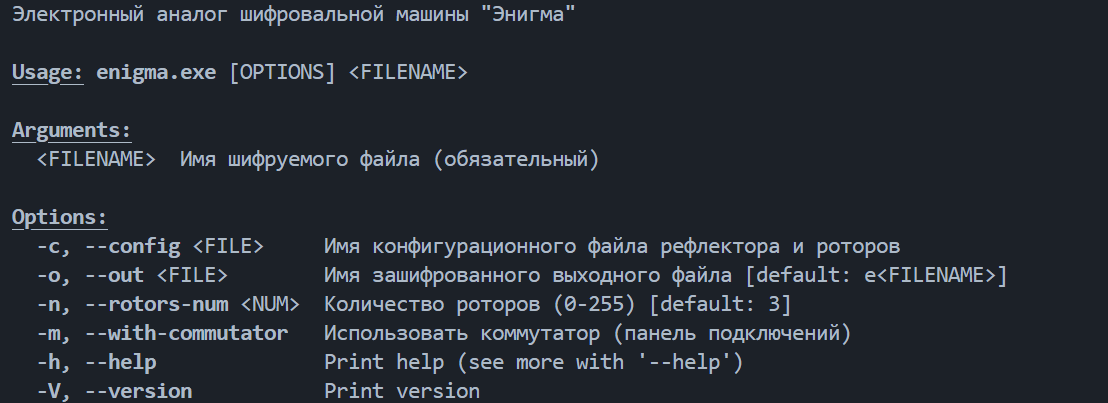
\includegraphics[width=1\linewidth]{images/prog_ex.png}
    \caption{Флаги CLI}
    \label{fig:prog}
\end{figure}

\begin{figure}[h]
    \centering
    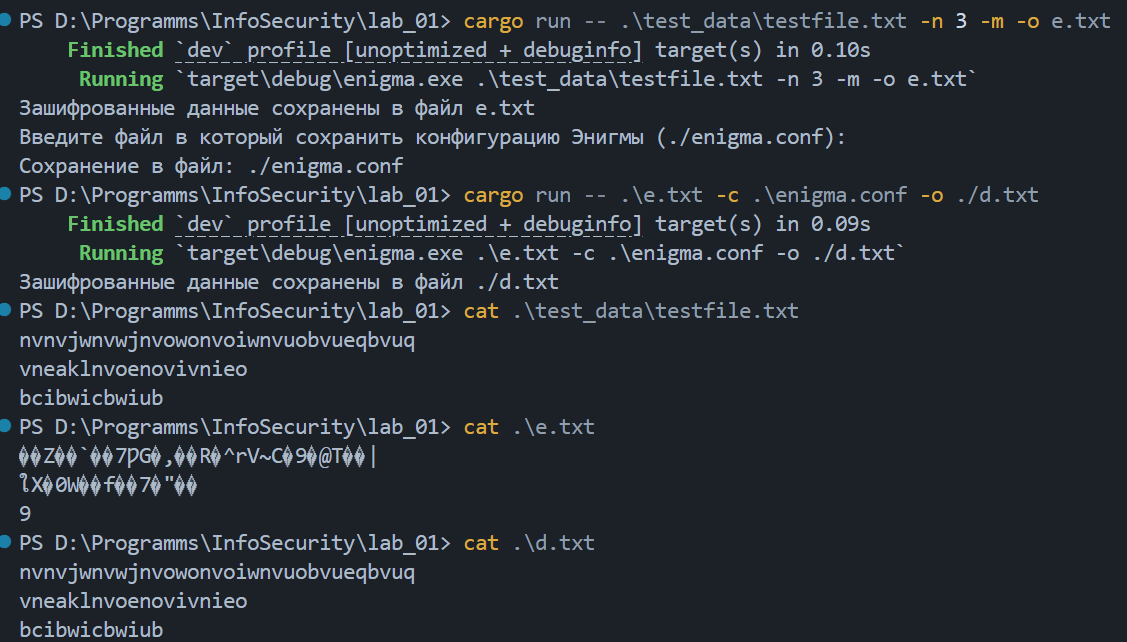
\includegraphics[width=1\linewidth]{images/image.png}
    \caption{Пример работы программы}
    \label{fig:prog}
\end{figure}

% \begin{figure}[h]
%     \centering
%     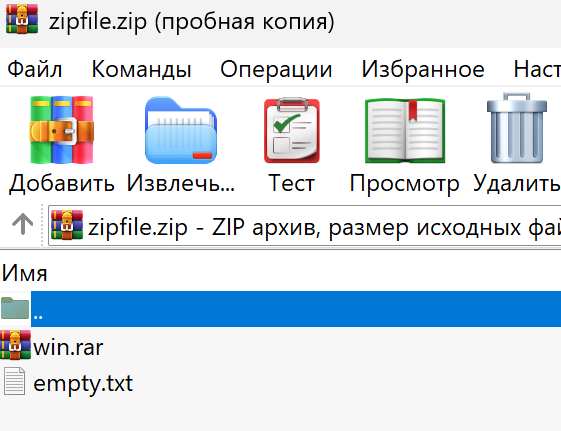
\includegraphics[width=0.6\linewidth]{images/z1.png}
%     \caption{Пример zip-файла}
%     \label{fig:prog}
% \end{figure}

% \begin{figure}[h]
%     \centering
%     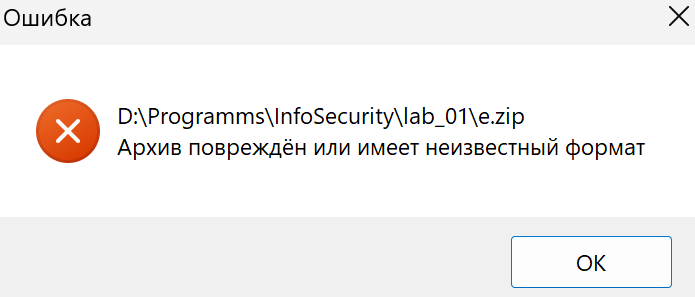
\includegraphics[width=0.6\linewidth]{images/ez.png}
%     \caption{Пример зашифрованного zip-файла}
%     \label{fig:prog}
% \end{figure}

% \begin{figure}[h]
%     \centering
%     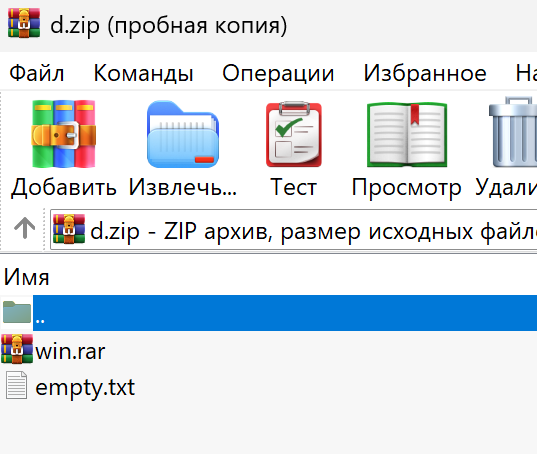
\includegraphics[width=0.6\linewidth]{images/dz.png}
%     \caption{Пример дешифрованного zip-файла}
%     \label{fig:prog}
% \end{figure}

\chapter*{ЗАКЛЮЧЕНИЕ}
\addcontentsline{toc}{chapter}{ЗАКЛЮЧЕНИЕ}

В результате лабораторной работы были изучены принципы работы шифровальной машины "Энигма", была реализована программа, способная шифровать и дешифровать файлы любого формата.
Были решены следующие задачи:

\begin{itemize}[label=---]
	\item проведен анализ работы шифровальной машина "Энигма";
	\item описан алгоритм шифрования;
	\item реализован описанный алгоритм;
\end{itemize}